\section{An Approximate Closed-Form Solution to the CON Dynamics}

\subsection{Approach}\label{sub:con:cfa:approach}
To predict future system states, we need to integrate the ODE in Eq.~\eqref{eq:con:con_dynamics}, with the solution given by $y(t_{k+1}) = y_{t_k} + \int_{t_k}^{t_{k+1}} f(y(t'), u(t')) \, \mathrm{d}t'$.
Unfortunately, a closed-form solution for the nonlinear dynamics $f(y, u)$ does not (yet) exist. Therefore, we traditionally need to revert to (high-order) numerical \gls{ODE} solvers that are computationally very expensive and introduce additional memory overhead~\citep{kidger2021neural}. This considerably increases the training time of models involving such continuous-time dynamics.
While the computational time can be reduced by increasing the (minimum) time step of the integrator, this comes at the expense of an integration error, and we lose (part of) the theoretical guarantees and practical characteristics that the nominal \gls{ODE} provides.
In this work, we take an alternative approach by splitting the problem into (i) decoupled linear dynamics that can be cheaply and precisely integrated using a closed-form solution and (ii) the residual, coupled nonlinear dynamics, which we integrate numerically at a slower time scale:

\begin{equation}\label{eq:con:con_split_linear_terms}
\begin{split}
    \ddot{x}(t) = \underbrace{F -\kappa x(t) - d \, \dot{x}(t)}_{f_{\ddot{x}, \mathrm{ld}}(y): \, \text{decoupled, linear dynamics}} + \underbrace{g(u(t)-(K-\kappa) x(t) - (D-d) \, \dot{x}(t) - \tanh(W x(t) + b)}_{f_{\ddot{x}, \mathrm{nld}}(y, u): \: \text{coupled, nonlinear dynamics}}
\end{split}
\end{equation}
where $\kappa = \mathrm{diag}(K_{11} \dots K_{nn})$, $d = \mathrm(D_{11} \dots D_{nn})$ are the diagonal components of the stiffness and damping matrices, respectively, and $F \in \mathbb{R}^{n}$ is a constant, external forcing term on the oscillators.

For a short-time-interval $\delta t$, we now approximate \eqref{eq:con:con_split_linear_terms} as
\begin{equation}\label{eq:con:con_approx}
    \ddot{x}(t_k+\delta t) \approx f_{\ddot{x}, \mathrm{ld}}(y(t_k+\delta t), F(t_k)) 
    \qquad \text{with  }
    F(t_k) =  -f_{\ddot{x}, \mathrm{nld}}(y(t_k), u(t_k)).
    % f_\mathrm{ext}(t_k) = -g(u(t_k))-(K-\kappa) x(t_k) - (D-d) \, \dot{x}(t_k) - \tanh(W \, x(t_k) + b)
\end{equation}
For a scalar \nth{2}-order, linear \gls{ODE} of form $\dot{y}_i = f_{\mathrm{ld},i}(x(t'), F(t_k))$, a well-known, closed-form solution~\citep{Pas2023damped} exists.
We exploit this characteristic by formulating the approximate solution as 
\begin{equation}\label{eq:con:cfa_con}
    y(t_k + \delta t) \approx \, f_\mathrm{CFA-CON}(y(t_k), u(t_k)) =  y(t_k) + \int_{t_k}^{t_k + \delta t} f_{\mathrm{ld}}(y(t'), F(t_k)) \, \mathrm{d}t'
\end{equation}
and denote $f_\mathrm{CFA-CON}: \mathbb{R}^n \times \mathbb{R}^m \to \mathbb{R}^n$ as the \gls{CFA-CON} model.
The implicit assumption behind \eqref{eq:con:con_approx} is that $f_{\ddot{x}, \mathrm{ld}}(y) \succ f_{\ddot{x}, \mathrm{nld}}(y, u)$ (i.e., the linear, decoupled dynamics dominate the nonlinear, coupled, time-varying dynamics).

% \begin{equation}
%     y_i (t_{k+1}) 
%     = \begin{bmatrix}
%         x_i(t_{k+1})\\
%         \dot{x}_i(t_{k+1})
%     \end{bmatrix} 
%     = \begin{bmatrix}
%         \left ( c_{1,i} \, \cos(\beta_i \, \delta t) +  c_{2,i} \sin(\beta_i \delta t) \right ) \, e^{-\alpha_i \, \delta t} + \frac{f_{\mathrm{ext},i}}{\kappa_i}\\
%         -\left ( (c_{1,i} \alpha_i - c_{2,i} \beta_i) \, \cos(\beta_i \delta t) +  (c_{1,i} \beta_i + c_{2,i} \alpha_i) \, \sin(\beta_i \delta t) \right ) \, e^{-\alpha_i \, \delta t}
%     \end{bmatrix},
% \end{equation}
% exists, where $\delta t = t_{k+1} - t_k$, $c_{1,i}, c_{2,i} \in \mathbb{R}$ are scalar integration constants dependent on $y_i(t_k), F_{i}(t_k)$, and $\alpha_i, \beta_i \in \mathbb{R}^+$ are real positive constants. Please refer to Appendix~\ref{apx:sec:con_cfa} for more details on the determination of the constants and the implementation.


\subsection{Closed-Form Solution to a Forced Harmonic Oscillator}
As introduced in \eqref{eq:con:harmonic_oscillator}, we consider the linear dynamics of a 1D forced harmonic oscillator with state $y_{i} = \begin{bmatrix}
    x_i & \dot{x}_i
\end{bmatrix} \in \mathbb{R}^2$
\begin{equation}
    \dot{y}_i = \begin{bmatrix}
        \frac{\mathrm{d} x_i}{\mathrm{d} t}\\
        \frac{\mathrm{d} \dot{x}_i}{\mathrm{d} t}
    \end{bmatrix} = f_{\mathrm{ld},i}(y_{i}, F_{i}) = \begin{bmatrix}
        \dot{x}_i\\
        F_i(t) - \kappa_i \, x_i(t) - d_i \, \dot{x}_i(t)
    \end{bmatrix},
\end{equation}
where $F_i(t) \in \mathbb{R}$ is the externally applied force acting on the oscillator.

The characteristic equation for the unforced dynamics (i.e., $F_i(t) = 0)$ can be stated as~\citep{Pas2023damped}
\begin{equation}
    \lambda^2 + 2 \, \zeta_i \, \omega_{\mathrm{n},i}  \, \lambda + \omega_{\mathrm{n},i}^2 = 0,
    \qquad
    \text{with the solutions} \:
    \lambda_{1,2} = -\zeta_{i} \,  \omega_{\mathrm{n},i} \pm \omega_{\mathrm{n},i} \, \sqrt{\zeta_{i}^2 - 1},
\end{equation}
 where $\omega_{\mathrm{n},i} = \sqrt{\kappa_i}$ and $\zeta_i = \frac{d_i}{2 \, \sqrt{\kappa_i}}$ are the natural frequency and the damping factor of the $i$th homogeneous oscillator, respectively.
 This harmonic oscillator exhibits three regimes: underdamped ($\zeta_i < 1$), critically damped ($\zeta_i = 1$), and overdamped regime ($\zeta_i > 1$).

 We approximate the forcing using the Heavyside function $H(t)$: $F_i(t) = F_{i}(t_k) \, H(t)$, where $F_{i}(t_k)$ is the constant external forcing as computed by \eqref{eq:con:con_approx}. The solution for $\zeta_i \neq 1$ is given by~\citep{Pas2023damped}
\begin{equation}\label{eq:con:harmonic_oscillator_closed_form}
    y_i (t_{k+1}) 
    = \begin{bmatrix}
        x_i(t_{k+1})\\
        \dot{x}_i(t_{k+1})
    \end{bmatrix} 
    = \begin{bmatrix}
        \left ( c_{1,i} \, \cos(\beta_i \, \delta t) +  c_{2,i} \sin(\beta_i \, \delta t) \right ) \, e^{-\alpha_i \, \delta t} + \frac{F_{i}}{\kappa_i}\\
        -\left ( (c_{1,i} \alpha_i - c_{2,i} \beta_i) \, \cos(\beta_i \, \delta t) +  (c_{1,i} \beta_i + c_{2,i} \alpha_i) \, \sin(\beta_i \, \delta t) \right ) \, e^{-\alpha_i \, \delta t}
    \end{bmatrix},
\end{equation}
where $\delta t = t_{k+1} - t_k$, $\alpha_i = \zeta_i \, \omega_{\mathrm{n},i}$, and $\beta_i = \omega_{\mathrm{n},i} \, \sqrt{1-\zeta_i^2}$.
After enforcing the initial conditions $x_i(t_k), x_i(t_k)$, the integration constants
\begin{equation}
    c_{1,i} = x_i(t_k) - \frac{F_{i}(t_k)}{\kappa_i},
    \qquad
    c_{2,i} = - 2 \, j \, \frac{\dot{x}_i(t_k) + \alpha_i \, \left (x_i(t_k) - \frac{F_{i}}{k_i} \right )}{\Delta \lambda_i},
\end{equation}
can be identified with $\Delta \lambda_i = \lambda_{i,2} - \lambda_{i,1} = - 2 \, \beta_i \, j$, where $j$ is the imaginary value.
While we could derive the solution for the critically damped case $d_i < 2 \sqrt{\kappa_i}$ separately, we instead approximate it in our network dynamics with \eqref{eq:con:harmonic_oscillator_closed_form} by setting
$\Delta \lambda_i \cong \begin{cases}
    \mathrm{sign}(-2 \, \beta_i \, j) \, \epsilon   & |2 \, \beta_i \, j| < \epsilon \\
    - 2 \, \beta_i \, j & |2 \, \beta_i \, j| \geq \epsilon
\end{cases}$, where $\epsilon \in \mathbb{R}^+ \ll 1$ is a small, positive value.

\subsection{Algorithmic Implementation}
We can now leverage the closed-form solution to the evolution of a single, decoupled damped harmonic oscillator of \eqref{eq:con:harmonic_oscillator_closed_form} to solve the integral in \eqref{eq:con:cfa_con}
\begin{equation}\label{eq:con:cfa:full_con_cfa_dynamics}
\begin{split}
    y(t_{k+1}) \approx& \: f_\mathrm{CFA-CON}(y(t_k), u(t_k)),\\
    \begin{bmatrix}
        x(t_{k+1})\\ \dot{x}(t_{k+1})
    \end{bmatrix} \approx& \: \begin{bmatrix}
        \left ( c_{1} \odot \cos(\beta \, \delta t) +  c_{2} \odot \sin(\beta \, \delta t) \right ) \odot e^{-\alpha \, \delta t} + \frac{F(t_k)}{\kappa}\\
        -\left ( (c_{1} \odot \alpha - c_{2} \odot \beta) \, \cos(\beta \, \delta t) +  (c_{1} \odot \beta + c_{2} \odot \alpha) \, \sin(\beta \, \delta t) \right ) \odot e^{-\alpha \, \delta t}
    \end{bmatrix},
\end{split}
\end{equation}
with
\begin{equation}
\begin{split}
    \kappa = \mathrm{diag}(K_{11} \dots K_{nn}), \quad d = \mathrm(D_{11} \dots D_{nn}), \quad \omega_\mathrm{n} = \sqrt{\kappa}, \quad \zeta = \frac{d}{2 \sqrt{\kappa}},\\
    F(t_k) = g(u(t_k)) - (K - \kappa) \, x(t_k) - (D-d) \, \dot{x}(t_k) - \tanh \left (Wx(t_k)+b \right ),\\
    \delta t = t_{k+1} - t_k, \qquad \alpha = \zeta \odot \omega_\mathrm{n}, \qquad \beta = \omega_\mathrm{n} \: \sqrt{1-\zeta^2},\\
    c_{1} = x(t_k) - \frac{F(t_k)}{\kappa}, \qquad
    c_{2} = \frac{1}{\beta} \, \left ( \dot{x}(t_k) + \alpha \odot \left (x(t_k) - \frac{F(t_k)}{\kappa} \right ) \right ).
\end{split}
\end{equation}
We summarize the approach of integrating/rolling out the \gls{CFA-CON} dynamics in Algorithm~\ref{alg:con:con_cfa}.

\begin{algorithm}
\caption{Rollout of \gls{CFA-CON}.}\label{alg:con:con_cfa}
\hspace*{\algorithmicindent} \textbf{Inputs:} initial state $y(t_0)$, input sequence $\{u(t_0), \dots u(t_k), \dots u(t_N) \}$\\
\hspace*{\algorithmicindent} \textbf{Outputs:} state sequence $\{y(t_0), \dots y(t_k), \dots y(t_N) \}$
\begin{algorithmic}[1]
    \State $k \gets 0$
    % \For{\texttt{<some condition>}}
    %     \State \texttt{<do stuff>}
    % \EndFor
    \While{$k \leq N$}
        \State $(x(t_k), \dot{x}(t_k)) \gets y(t_k)$
        \State $F(t_k) \gets g(u(t_k)) - (K - \kappa) \, x(t_k) - (D-d) \, \dot{x}(t_k) - \tanh \left (Wx(t_k)+b \right )$
        \State $\omega_\mathrm{n}, \: \zeta \gets \sqrt{\kappa}, \: \frac{d}{2 \sqrt{\kappa}}$ \Comment{Compute the characteristics of the decoup. harm. oscillators.}
        \State $\alpha, \: \beta  \gets \zeta \odot \omega_\mathrm{n}, \: \omega_\mathrm{n} \: \sqrt{1-\zeta^2}$
        \State $c_{1} \gets x(t_k) - \frac{F(t_k)}{\kappa}$  \Comment{Compute integration constants using initial conditions.}
        \State $c_{2} \gets \frac{1}{\beta} \, \left ( \dot{x}(t_k) + \alpha \odot \left (x(t_k) - \frac{F(t_k)}{\kappa} \right ) \right )$
        \State $\delta t = t_{k+1} - t_k$  \Comment{Set time step.}\\
        \Comment{Update state with approximated closed-form solution.}
        \State $x(t_{k+1}) \gets  \left ( c_{1} \odot \cos(\beta \, \delta t) +  c_{2} \odot \sin(\beta \, \delta t) \right ) \odot e^{-\alpha \, \delta t} + \frac{F}{\kappa}$
        \State $\dot{x}(t_{k+1}) \gets -\left ( (c_{1} \odot \alpha - c_{2} \odot \beta) \, \cos(\beta \, \delta t) +  (c_{1} \odot \beta + c_{2} \odot \alpha) \, \sin(\beta \, \delta t) \right ) \odot e^{-\alpha \, \delta t}$
        \State $k \gets k+1$  \Comment{Update time index.}
    \EndWhile
\end{algorithmic}
\end{algorithm}

\subsection{Approximation Bounds for CFA-CON}
Lemma~\ref{lemma:con:con_cfa_bounds_lemma} demonstrates how, for the particular case of no external input and linearly decoupled oscillators (which we are always free to choose), we can establish bounds on the approximation error when using the closed-form solution instead of the ground-truth coupled oscillator dynamics.

\begin{lemma}\label{lemma:con:con_cfa_bounds_lemma}
    Suppose that the network is unforced with $g(u(t)) = 0$ and that $K = \mathrm{diag}(\kappa_1, \dots, \kappa_n)$, $D = \mathrm{diag}(d_1, \dots, d_n)$ such that the oscillators are not linearly coupled. Then, given any $t \geq 0$, and the initial state $y(0) \in \mathbb{R}^{2n}$, the error between the continuous dynamics $\ddot{x}(t)$ of \eqref{eq:con:con_dynamics} and the approximated dynamics $\hat{\dot{x}}(t)$ in \eqref{eq:con:con_approx}, is bounded by $\lVert \ddot{x}(t) - \hat{\ddot{x}}(t) \rVert \leq 2$. 
\end{lemma}
\begin{proof}
    \eqref{eq:con:con_dynamics}, \eqref{eq:con:con_approx} and $F =  -f_{\ddot{x}, \mathrm{nld}}(y(0), 0)$ give us
    \begin{equation}
    \begin{split}
        \lVert \ddot{x}(t) - \hat{\ddot{x}}(t) \rVert =& \left (f_{\ddot{x},\mathrm{ld}}(y(t), 0) + f_{\ddot{x},\mathrm{nld}}(y(t), 0) \right ) - f_{\ddot{x},\mathrm{ld}}(y(t), F),\\
        =& \: -K x(t) -D \dot{x} -\tanh(W x(t) + b) + K x(t) + D \dot{x} + \tanh(W x(0) + b),\\
        =& \: \lVert -\tanh(W x(t) + b) + \tanh(W x(0) + b) \rVert
        \: \leq \: 2.
    \end{split}
    \end{equation}
    
\end{proof}

\subsection{Empirical Evaluation of Approximation Error}
In Table~\ref{tab:con:cfa_evaluation}, we present a comparison of \gls{CFA-CON} with several other strategies for integrating nonlinear dynamics, such as \gls{CON}.
Following the implicit assumption made in the concept for the closed-form approximation (i.e., Sec.~\ref{sub:con:cfa:approach}), we consider the case of $g(u) = 0$, $K = \mathrm{diag}(\kappa_1, \dots, \kappa_n)$ and $D = \mathrm{diag}(d_1, \dots, d_n)$ but with the hyperbolic coupling between the oscillators active (i.e., a full $W$ matrix).
Integrating the dynamics at a very small time step (i.e., $\delta t = \num{5e-5}~\si{s}$) with a high-order \gls{ODE} solver would give us a very accurate solution, but this is computationally infeasible in practice. We, therefore, regard this as the upper bound on the accuracy of the solution.
A feasible solution would be to implement either a high-order solver such as Tsit5 at a larger integration time-step, e.g., $\delta t = \num{1e-1}~\si{s}$) or a low-order solver with a slightly smaller integration time step, e.g., $\delta t = \num{5e-2}~\si{s}$). Therefore, we also benchmark these options.
We also benchmark an implementation specialized on the underdamped case (i.e., $\zeta_i <1$): \gls{CFA-UDCON}. This specialized implementation allows us to avoid using complex numbers in the algorithm and reduces the number of computations necessary for calculating the approximated solution.
As a result, we see a considerable increase in the sim-time to real-time factor.

\begin{figure}[ht]
    \centering
    \subfigure[Positions]{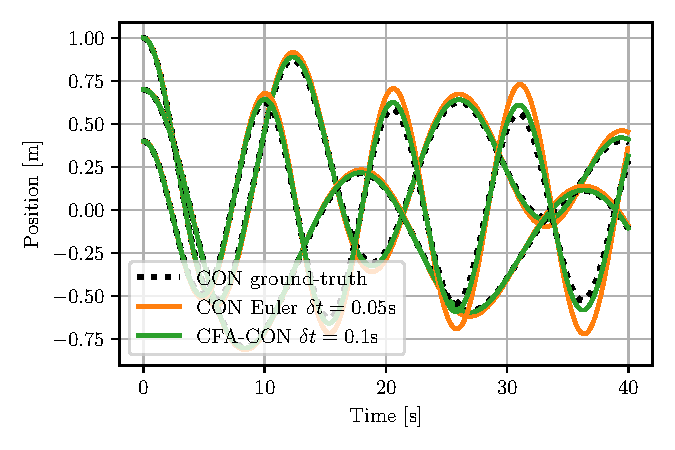
\includegraphics[width=0.49\textwidth, trim={5, 5, 5, 5}]{con/figures/results/cfa/coupled_oscillator_position.pdf}}
    % \hfill
    \subfigure[Velocities]{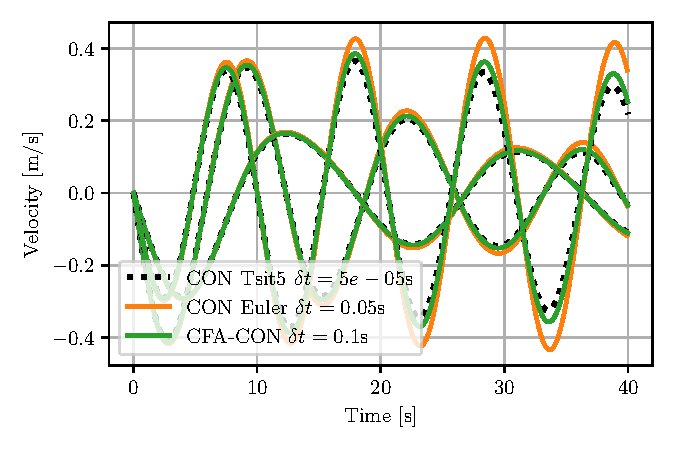
\includegraphics[width=0.49\textwidth, trim={5, 5, 5, 5}]{con/figures/results/cfa/coupled_oscillator_velocity.pdf}}
    \caption{Analysis of approximation error of CFA-CON: we compare the ground-truth solution of a \SI{40}{s} rollout of the \gls{CON} network consisting of three oscillators ($n=3$) with the \emph{CFA-CON} executed at a time step of $\delta t = \SI{0.1}{s}$ and a solution generated by integrating the \gls{ODE} at a time step of $\delta t = \SI{0.05}{s}$ with the Euler method.}
    \label{fig:con:cfa_con_comparison}
\end{figure}

\subsubsection{Integration error} 
We perform the integration error benchmark over $100$ different network configurations, all consisting of $50$ oscillators ($n=50$): First, we sample the natural frequency of the $i$th oscillator from a uniform distribution as $\omega_{\mathrm{n},i} \sim \mathcal{U}(\SI{0.05}{Hz}, \SI{0.5}{Hz})$, then we sample $\kappa_i \sim \mathcal{U}(\SI{0.2}{N\per m}, \SI{2}{N \per m})$ such that $K = \mathrm{diag}(\kappa_1, \dots, \kappa_n) \succ 0$, which lets us determine each mass $m_i = \frac{\kappa_i}{\omega_{\mathrm{n},i}^2}$.
Next, the damping ratio is determined as $\zeta_i \sim \mathcal{U}(0.1, 0.9)$ and $\zeta_i \sim \mathcal{U}(0.1, 2.0)$ for the underdamped and general case, respectively. As a result, $D = \mathrm{diag}(d_1, \dots, d_n) \succ 0$ with $d_i = 2 \, \zeta_i \, \sqrt{m_i \, \kappa_i}$ given.
Finally, by leveraging the Cholesky decomposition, we sample a $W \succ 0$  and $b_i \sim \mathcal{U}(-1, 1)$.
We compute the estimation error of all integrated trajectories with respect to the high-precision solution (i.e., Tsitouras' 5/4 method (Tsit5) at $\delta t = \num{5e-4}~\si{s}$).
For this, we compute the \gls{RMSE} for each \SI{60}{s} trajectory and then take the mean and standard deviation across the $100$ different network configurations.

\subsubsection{Simulation-Time to Real-Time Factor} 
The simulation vs. real-time factor is computed as the simulated rollout duration per second of computational time. For this, we let each method simulate a \SI{60}{s} trajectory for $100$ times and record the minimum run time on an Intel Core i7-10870H CPU (single core) over $10$ trials. Because of computational constraints, we simulated the trajectory  with the high-precision Tsit5 solver only $5$ times. 


\subsubsection{Results}
We also provide qualitative results for the integration accuracy in Fig.~\ref{fig:con:cfa_con_comparison}
The results in Table~\ref{tab:con:cfa_evaluation} show that \gls{CFA-CON} is \SI{30}{\percent} more accurate than the Euler integrator at half of the speed. Comparing against the Tsit5 integrator, \gls{CFA-CON} exhibits a 1.56x speed increase while being significantly less accurate.
For the underdamped case with $\zeta < 1$, the specialized implementation \gls{CFA-UDCON} is \SI{14.8}{\percent} faster and at the same time \SI{32}{\percent} more accurate than the Euler integrator. Furthermore, \gls{CFA-UDCON} is 3.7x faster and significantly less accurate than the Tsit5 integrator.
We can conclude that in the pure rollout setting (i.e., no backpropagation involved) for a generic \gls{CON}, the \gls{CFA-CON} does not show clear advantages to an appropriately tuned Euler or Tsit5 solver. However, the specialized version \gls{CFA-UDCON} demonstrates a 2.4x speed-up at no reduction of accuracy vs. \gls{CFA-CON} for underdamped oscillator networks.


\begin{table}[ht]
    \centering
    \begin{scriptsize}
    \begin{tabular}{c c c c r }
         \toprule
         \textbf{Method} & \textbf{RMSE} [m] $\downarrow$ & \textbf{RMSE} $\zeta < 1$ [m] $\downarrow$ & \textbf{Complexity} $\downarrow$ & \thead{\textbf{$\frac{\text{Sim. time}}{\text{Real time}}$}} $\uparrow$ \\
         \toprule
         \makecell{\gls{CON} with Tsit5\\ at $\delta t = \num{5e-5}~\si{s}$} & n/a & n/a & $\mathcal{O} \left (\frac{n^{\log_2 7} p h}{\delta t} \right) = \mathcal{O}(\num{3.5e11})$ & $5.68$x\\
         \midrule
         \makecell{\gls{CON} with Tsit5\\ at $\delta t = \num{1e-1}~\si{s}$} & $\mathbf{\num{5e-5} \pm \num{1e-5}}$ & $\mathbf{\num{8e-6} \pm \num{1e-5}}$ & $\mathcal{O} \left (n \frac{n^{\log_2 7} p h}{\delta t} \right) = \mathcal{O}(\num{1.8e8})$ & $11310$x\\
         \midrule
         \makecell{\gls{CON} with Euler\\ at $\delta t = \num{5e-2}~\si{s}$} & $\num{0.010} \pm \num{0.003}$ & $\num{0.022} \pm \num{0.005}$ & $\mathcal{O} \left (\frac{n^{\log_2 7} h}{\delta t} \right) = \mathcal{O}(\num{7.1e7})$ & $36500$x\\
         \midrule
         \makecell{\gls{CFA-CON} (our)\\ with $\delta t = \num{1e-1}~\si{s}$} & $\num{0.007} \pm \num{0.002}$ & $\num{0.015} \pm \num{0.003}$ & $\mathcal{O} \left (\frac{n^{\log_2 7} h}{\delta t} \right) = \mathcal{O}(\bf{\num{3.5e7}})$ & $17680$x\\
         \midrule
         \makecell{\gls{CFA-UDCON} (our)\\ with $\delta t = \num{1e-1}~\si{s}$} & n/a & $\num{0.015} \pm \num{0.003}$ & $\mathcal{O} \left (\frac{n^{\log_2 7} h}{\delta t} \right) = \mathcal{O}(\bf{\num{3.5e7}})$ & $\mathbf{41900}$\textbf{x}\\
         \bottomrule
    \end{tabular}
    \end{scriptsize}
    \vspace{0.5cm}
    \caption{Benchmarking of various methods for integrating the \gls{CON} dynamics.
    The \gls{RMSE} is computed with respect to the Tsitouras' 5/4 method (Tsit5) (i.e., extremely high accuracy but also extremely high computational complexity). 
    We denote with $n$ the number of oscillators in the network (in this case $n=50$), with $p$ the order of the numerical \gls{ODE} solver, and with $\delta t$ the time-step.
    When stating the complexity, we refer to $h = t_N-t_0$ as the rollout horizon in seconds. In this case, we report the results for a horizon of $h = \SI{60}{s}$.
    The \gls{RMSE} column states the \gls{RMSE} of the various integration strategies with respect to the \emph{CON with Tsit5 at $\delta t = \num{5e-5}$s} solution, which we consider to be the ground-truth.
    The \emph{RMSE $\zeta < 1$} computes the same metrics, but this time for a dataset that contains only underdamped oscillators.
    The \emph{$\frac{\text{Sim. time}}{\text{Real time}}$} column states the ratio between the duration of the simulation achieved (in seconds) per second of real-time (i.e., computational time).
    We report the mean and standard deviation of the \gls{RMSE} over $100$ different network configurations.
    }
    \label{tab:con:cfa_evaluation}
\end{table}